% =====================================================================
% SUPPLEMENTARY NOTE 8 — X13, reproducible marker signatures.
%
% SOURCES. axw1008/docs/paper/x13_marker_reproducibility.csv and its null
% file, written by src/scripts/marker_reproducibility.py (job 61726250).
% The protocol is that script's docstring. The test uses the COUNTS, not
% the latent: nothing in it depends on the model.
%
% AW's ruling on the register: a clear refutation of the marker half of
% HECA's claim, no hedge, and no speculation about why they found
% otherwise. The cycle-coverage half of their complaint applies to this
% corpus and is said so.
% =====================================================================

\section{Marker signatures reproduce across cohorts}
\label{note:markers}

The largest prior atlas of the endometrium states that earlier atlases
lack reproducible marker gene signatures, consensus annotation, and even
cycle coverage \citep{mareckova2024heca}. The marker half of that claim is
testable here and in no single cohort, because testing it needs
independently annotated cohorts measured on one gene space, which is what
the pooled corpus is. This note gives the test and its result. The test
uses the count matrices and the studies' own annotations and never touches
the model, so it is a statement about the corpus rather than about
\elaj{}.

\subsection{The test}

Two studies annotated their own cells at the family level,
\texttt{duempelmann\_2026} with 132{,}259 held-out cells and
\texttt{marecko\_2024} with 44{,}544, each labelling stromal, epithelial,
endothelial and immune. Within each study and for each family, a
one-against-rest signature was derived over every gene the study measured:
the standardised mean difference, on log-transformed counts per ten
thousand, between the family's cells and the rest of that study's cells.
The statistic is deterministic, runs in two sparse passes, and is monotone
in the $t$-statistic a marker ranking would use. The two studies' own labels
were used rather than the transferred ones, because a signature derived
from a transferred label is a reading of a prediction, and agreement
between two such signatures would partly measure whether the transfer was
consistent rather than whether the biology is.

Every comparison was restricted to the 13{,}034 genes both studies'
panels measured. A study's panel does not measure every gene in the
vocabulary, and an unmeasured gene arrives as a structural zero; compared
without the restriction, a gene absent from one panel reads as a confident
non-marker there rather than as unknown, which would depress every
agreement by an amount that depends on how different the two panels are.
Agreement was then scored two ways per family: the number of genes shared
between the two studies' top hundred, and the Spearman rank correlation
between the two signatures over all 13{,}034 genes. The null shuffles family
labels within each study, keeping each study's family proportions, and
reruns the whole comparison; twenty shuffles were run. The overlap of two
top-hundred lists has a floor set by the list length and the gene count,
and the null is what measures it.

\subsection{The result}

Table~\ref{stab:x13} and Supplementary Figs.~\ref{sfig:x13-overlap}
and~\ref{sfig:x13-rho} give the result. The two cohorts share 76 of each
other's top hundred stromal marker genes, 69 epithelial, 69 endothelial and
61 immune, at rank correlations over the full gene space of 0.8256, 0.8121,
0.7129 and 0.8053. Across twenty within-study label shuffles no family ever
shares more than three genes and no rank correlation leaves the interval
$-0.048$ to $+0.067$. Two cohorts that sequenced different people, in
different laboratories, on different platforms, and annotated their cells
independently, rank the same genes at the top for every family once they
are read on one gene space. On the marker half of the claim, the
signatures reproduce.

\begin{table}[t]
\centering
\caption[Marker reproducibility by family]{\textbf{Agreement between the
two cohorts' per-family marker signatures, against twenty within-study
label shuffles.} Jaccard is the top-hundred overlap over the union of the
two lists.}
\label{stab:x13}
\footnotesize
\resizebox{\textwidth}{!}{% GENERATED by figures/scripts/supp_figures.py. Do not edit by hand.
\begin{tabular}{@{}lrrrrrr@{}}
\toprule
family & shared genes & top-100 overlap & Jaccard & Spearman $\rho$ & null max overlap & null $\rho$ range (20 shuffles) \\
\midrule
stromal & 13034 & 76 & 0.613 & 0.8256 & 2 & $-$0.036 to +0.046 \\
epithelial & 13034 & 69 & 0.527 & 0.8121 & 3 & $-$0.032 to +0.048 \\
endothelial & 13034 & 69 & 0.527 & 0.7129 & 3 & $-$0.043 to +0.067 \\
immune & 13034 & 61 & 0.439 & 0.8053 & 2 & $-$0.048 to +0.042 \\
\bottomrule
\end{tabular}
}
\end{table}

\begin{figure}[t]
\centering
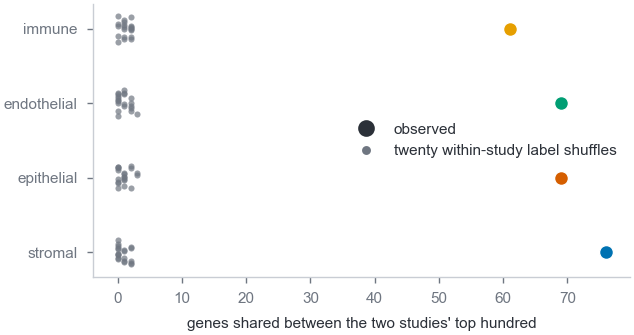
\includegraphics[width=.65\textwidth]{figures/x13_overlap_vs_null.png}
\caption[Top-hundred overlap against the null]{\textbf{Genes shared between
the two cohorts' top hundred, by family}, observed against twenty label
shuffles.}
\label{sfig:x13-overlap}
\end{figure}

\begin{figure}[t]
\centering
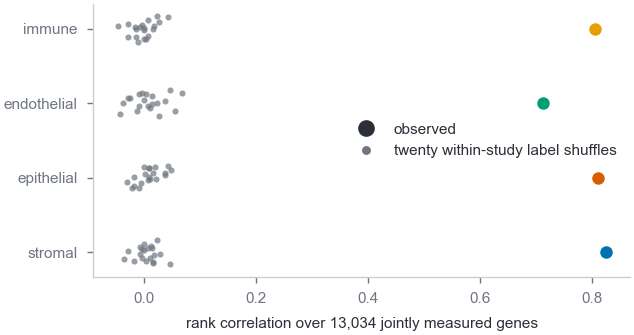
\includegraphics[width=.65\textwidth]{figures/x13_spearman_vs_null.png}
\caption[Rank correlation against the null]{\textbf{Rank correlation
between the two signatures over 13{,}034 genes, by family}, observed against
twenty label shuffles.}
\label{sfig:x13-rho}
\end{figure}

\subsection{What the test does not show}

It is one pair of cohorts, because only two studies in the corpus
annotated their own cells, and it is four families, because that is the
vocabulary the two share; whether finer cell types reproduce as well is
not answered here and would need the finer vocabularies reconciled first.
The restriction to jointly measured genes is what makes the comparison
fair and it is also a choice; a reader who compares the two cohorts on each
study's full panel will find lower agreement, and the difference is the
panels, not the biology. The other half of the prior atlas's complaint,
cycle coverage, applies to this corpus: phase labels come from three
studies and a cycle day from one, and the corpus is quoted against the
claim with that half conceded.
